\documentclass[a4paper,11pt]{report}

\usepackage{amsmath,amssymb,amsfonts,amsthm,ascmac, listings, courier}    % Typical maths resource packages
\usepackage{graphicx}                           % Packages to allow inclusion of graphics
\usepackage{hyperref}                           % For creating hyperlinks in cross references
\usepackage{bookmark}
\usepackage[authoryear]{natbib}                 % literature reference style
\usepackage[bf]{caption2}
\usepackage{listings}


 \lstset{
         basicstyle=\footnotesize\ttfamily, % Standardschrift
         %numbers=left,               % Ort der Zeilennummern
         numberstyle=\tiny,          % Stil der Zeilennummern
         %stepnumber=2,               % Abstand zwischen den Zeilennummern
         numbersep=5pt,              % Abstand der Nummern zum Text
         tabsize=2,                  % Groesse von Tabs
         extendedchars=true,         %
         breaklines=true,            % Zeilen werden Umgebrochen
         keywordstyle=\color{red},
    	 frame=b,         
 %        keywordstyle=[1]\textbf,    % Stil der Keywords
 %        keywordstyle=[2]\textbf,    %
 %        keywordstyle=[3]\textbf,    %
 %        keywordstyle=[4]\textbf,   \sqrt{\sqrt{}} %
         stringstyle=\color{white}\ttfamily, % Farbe der String
         showspaces=false,           % Leerzeichen anzeigen ?
         showtabs=false,             % Tabs anzeigen ?
         xleftmargin=17pt,
         framexleftmargin=17pt,
         framexrightmargin=5pt,
         framexbottommargin=4pt,         
         %backgroundcolor=\color{lightgray},
         showstringspaces=false      % Leerzeichen in Strings anzeigen ?              
 }
 
\lstloadlanguages{C}




% -------------------------------
% --- some layout definitions ---
% -------------------------------

% define topline
\usepackage[automark]{scrpage2}
\pagestyle{plain}
\automark{section}
\clearscrheadings
\ohead{\headmark}


% define citation style
\bibliographystyle{unsrt}

% define page size, margin size
\setlength{\headheight}{2\baselineskip}
\voffset=-3cm
\hoffset=-3cm
\textheight24cm
\textwidth16.5cm
\topmargin1cm
\oddsidemargin3cm
\evensidemargin3cm

% define line line spacing = 1.5
\renewcommand{\baselinestretch}{1.5}

% define second level for `itemizing'
\renewcommand{\labelitemii}{-}

%get all citing in bib file - fix bib running errorj
\nocite{*}



% --------------------------------------
% --------------------------------------
% --------------------------------------
% --- the structure the tex document ---
% ---  (this our recommendation) -------
% frontmatter:
%   - titlepage (mandatory),
%   - acknowledgement,
%   - abstract,
%   - table of contents (mandatory),
%   - list of abbreviations (not mandatory),
%   - list of figures (not mandatory),
%   - list of tables  (not mandatory) .
%
% body of the thesis (the structure ozf the thesis body is not mandatory, but the list of literature is mandatory):
%   - introduction,
%   - background
%   - system design
%   - implement
%   - result
%   - conclusion
%   - appendix (figures, tables).
%
% last page:
%   - declaration of authorship (mandatory).
% --------------------------------------
% --------------------------------------
% --------------------------------------

\begin{document}

% -------------------------------
% --- frontmatter: Title page ---
% -------------------------------

%\thispagestyle{empty}


\thispagestyle{empty}
%\parindent=1zw

\begin{center}

%\vspace{30mm}
\vspace{30mm}
%{\LARGE\bf LECTES: A Low Energy Consumption Time Estimation}\\ 
{\LARGE\bf An approach to fast malware classification with machine learning technique }\\ 
%\vspace{2mm}
%{\LARGE\bf malware's meta-data using machine learning %technique}\\%\vspace{5mm}
%\vspace{3mm}

%\vspace{2cm}
\vspace{10mm}

{\LARGE Pham Van Hung}\\
%\vspace{2cm}
\vspace{10mm}
{\Large Faculty of Environment and Information Studies}\\
\vspace{5mm}
{\LARGE Keio University}\\
\vspace{5mm}
{\Large 5322 Endo Fujisawa Kanagawa 252-0882}
{\Large JAPAN}\\
%\vspace{2cm}
\vspace{10mm}

{\Large\it  Submitted in partial fulfillment of the requirements} \\
\vspace{3mm}
{\Large\it  for the degree of Bachelor}\\

%\vspace{2cm}
\vspace{12mm}

\textbf{{\Large Advisors:}}\\
\vspace{5mm}
{\Large Professor Hideyuki Tokuda}\\
\vspace{2mm}
{\Large Professor Jun Murai}\\
\vspace{2mm}
{\Large Associate Professor Hiroyuki Kusumoto}\\
\vspace{2mm}
{\Large Professor Osamu Nakamura}\\
\vspace{2mm}
{\Large Associate Professor Kazunori Takashio}\\
%\vspace{2mm}
%{\Large Assistant Professor Noriyuki Shigechika}\\
\vspace{2mm}
{\Large Assistant Professor Rodney D. Van Meter III}\\
\vspace{2mm}
{\Large Associate Professor Keisuke Uehara}\\
\vspace{2mm}
{\Large Associate Professor Jin Mitsugi}\\
\vspace{2mm}
{\Large Lecturer Jin Nakazawa}\\
\vspace{2mm}
{\Large Professor Keiji Takeda}\\

%\vspace{1.5cm}
\vspace{10mm}

{\large Copyright\copyright  2011 Pham Van Hung}

\end{center}





\renewcommand{\baselinestretch}{1.7}
% -----------------------------
% --- frontmatter: Abstract ---
% -----------------------------
\newpage
\begin{center}

%%%%%%%%%%%%%%%%%%%%%%%%%%%%%%%%%%%%%%%%%%%%%%%%%%%%%%%%%%%%%%
% Abstract.
%%%%%%%%%%%%%%%%%%%%%%%%%%%%%%%%%%%%%%%%%%%%%%%%%%%%%%%%%%%%%%

\begin{Large}
{\bf Abstract of Bachelor Thesis} \\

\vspace{5mm}

{\bf An approach to fast malware classification with machine learning technique}
\end{Large}
\end{center}

\vspace{0.8cm}
 
  With the rapid increase of malware, it is important for malware analysis to classify unknown malware files into malware families. By doing so, the behavior and characteristics of malware will be identified accurately. In this paper, an approach was introduced to perform fast malware classification based on meta-data of malware's file. A machine learning technique called decision tree algorithm, is used to classify malware rapidly and correctly. Experimental results of the malware samples show that the system successfully determined some semantic malware similarities, especially showed their inner similarities in behavior and static malware characteristic.  \\

Keywords:

Malware, static analysis, decision tree.

\vspace{0.5cm}

\begin{flushright}
{\bf Pham Van Hung}\\
\vspace{2mm}
{\bf Faculty of Environment and Information Studies}\\
{\bf Keio University}\\
\end{flushright}



% -----------------------------
% --- frontmatter: Contents ---
% -----------------------------
\newpage
\tableofcontents
\clearpage


% ----------------------------------------------------
% --- frontmatter: List of Figures (not mandatory) ---
% ----------------------------------------------------
%\newpage
%\addcontentsline{toc}{section}{List of Abbreviations}
%\ohead%[]{LIST OF ABBREVIATIONS}
%\section*{List of Abbreviations}

\begin{tabular}{rp{0.2cm}lp{1cm}rp{0.2cm}l}
    DHT     & &  Distributed Hash Table   & & PIM     & &  Protocol Independent Multicast  \\
    MSDP     & &  Multicast Source Discovery Protocol                
\end{tabular}




% ----------------------------------------------------
% --- frontmatter: List of Figures (not mandatory) ---
% ----------------------------------------------------
\newpage
\addcontentsline{toc}{section}{List of Figures}
\ohead[]{\rightmark}
\listoffigures

% ---------------------------------------------------
% --- frontmatter: List of Tables (not mandatory) ---
% ---------------------------------------------------
\newpage
\addcontentsline{toc}{section}{List of Tables}
\listoftables

% -------------------------------
% --- main body of the thesis ---
% -------------------------------
\newpage
\setcounter{page}{1}    % start page numbering anew
\pagenumbering{arabic}  % page numbers in arabic style


\chapter{Introduction}\label{chap:1}

%INTRODUCTION
%
%
\section{Background}
Malware is a general word for all types of malicious software. Malware includes Virus, Trojan house, Back door, Worm, and other malicious software which are characterized by malicious code.
Because of the widespread use of the Internet, computer users face many dangerous propagations of malware. The modern malware's purpose is commonly illegal profit. For example, a large number of computers are infected by keylogger and $24.3$ billion USD is leveraged  by e-payment system losing \cite{keylogger}. In addition, According to 2010 Annual Security Report, on May 2010, tens of millions computer world wide were infected by email worm such as “I LOVE YOU”, “LOVE LETTER, “LOVEBUG”\cite{Symantec}. As a result tasks such as preventing, detecting, and removing malware are very important for network security.
	
\section{Malware analysis problem}	
This session will be a detailed introduction on malware analysis of security professionals. Malware analysis is the process of analysing the purpose and functionally of a malware. Malware analysis purpose is understanding of characteristics that all viruses in a family have in common and create a set of signatures in order to detect malwares. In addition, the knowledge about the purpose and functionally of a malware is important for removal.

Commonly, dynamic and static malware analysis have been applied. When new malware is detected, dynamic malware analysis technique executes malware in the Virtual Machine using ProcMon, RegShot, and other tools. These tools are used to identify the general behavioral analysis techniques such as network traffic analysis, file system, and other Window features such as service, process, and the registry. 

However, the dynamic techniques are susceptible to a variety of anti-monitoring defenses, as well as \emph{time bombs} or \emph{logic bombs} and can be slow and tedious to identify and disable code analysis techniques to unpack the code for examination \cite{georg}. Furthermore, it takes large amount of time to prepare malware analyzing environment to analyze malware such as virtual machine environment. However, some malware can not be executed in those kind of environment.

With the static malware analysis technique, researchers perform reverse engineering using IDA Pro and Ollydbg tool to analyze malware based on its structure in order to discover its purpose and functionality but it takes a lot of time to see the malware structure. 

Malware analysis is necessary to understand the behavior of malware. As a result, malware signature is created to effectively detect malware. Nevertheless, it wastes much time to find out the behavior and characteristic of malware.

With a vast amount of samples increasing day by day, it is harder for anti-virus industry and virus researchers to analyze malware without information of new malware. In order to reduce time of malware analysis, it is necessary to have an automatic malware classification system.

\section{Approach}

The thesis focused on two following issues:
\begin{itemize}
\item Automatically perform fast malware classification based on malware file's meta-data Use a machine learning technique, called decision tree algorithm to classify unknown malwares or subspecies rapidly and correctly.

\item Help researcher to understand which family malware belongs to and detect some semantic information about malware. 
\end{itemize}

For those reason, in this paper, an approach is proposed to perform fast malware classification based on malware's meta-data using machine learning technique known as decision tree.

\section{Thesis outline}
The rest of this thesis is structured as follows: \begin{itemize}
\item Chapter 2 describes malware meta-data, and method in the static classification of malware. Insight is provided to understand the purpose of method given in this research.
\item Chapter 3 presents the other malware static classification approach.
\item Chapter 4 gives approach, design and operation of malware classification system.
\item Chapter 5 mentions environment and implementation of static malware system.
\item Chapter 6 shows the system evaluation method and results. 
\item Summary, the conclusion and future work are presented in chapter 7
\end{itemize}


\chapter{Background}\label{chap:2}
This chapter presents the growth of malware, together with malware analysis technique. Afterwards, it introduces malware categories and the way of Virus total service to detect malware name defined by anti-virus vendor. Finally, there are problems of using malware name to detect semantic meaning of malware. 
%RELATED WORK
%
%
\section{Growth of malware attack}
Malware can self-replicate recursively. For example, Mota is a kind of worm that spreads itself by sending spam email to address harvested from local machine \cite{mota}. In addition, Downadup is a malware that receives and executes file through a peer-to-peer system by communication between computers\cite{downadup}. Malware infects system and spreads to the other systems by communication tools. Recently, malware has damaged system and sent the copy of itself to the other systems through Internet.

Since the rise of widespread broadband Internet access, the number of malware samples have rapidly increased. According to the report issued by Kaspersky's research team, 205 million pieces of malware were detected and neutralized \cite{kaspersky1}. In addition, in 2010 the number of malware samples increased by 20 millions \cite{kaspersky}.Figure \ref{fig:kaspersky} shows the increase of malware from 2003 to 2009 by Kaspersky Lab. As a result of the fast growth malware, malware is still a huge problem in Internet security and network connectivity. 
\begin{figure}[h!]
\centering
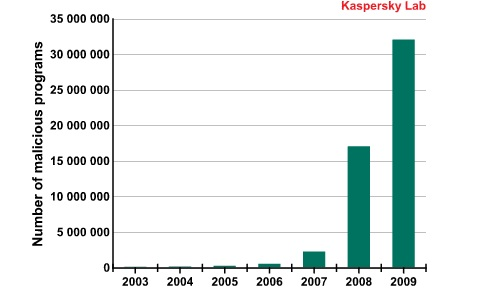
\includegraphics[width=1\textwidth]{graph/kapersky.jpg}
\caption{Number of malicious program}\cite{kaspersky}
\label{fig:kaspersky}
\end{figure}

At this time, malware is easy created by Malware Creation Tool, known a program which is by attacker to generate malware\cite{Microsoft}. In addition, unlike early attack tools implementing one type of attack, such tools now can be changed quickly by upgrading or replacing their code. This causes rapidly evolving attacks and, at the extreme, results in polymorphic tools that self-evolve, change with each active instance of the attack. Therefore, a large amount of malware have challenged anti-virus vendor and researcher in effective analysis.

\section{Malware avoidance technique}

At the present time, malware is implemented with avoidance technique in order to invalidate static signature based method by anti-virus software and make analysis process more complicated. Avoidance technique can change malware signature and syntax without changing the behaviors of malware. The avoidance technique consists of obfuscating code and packing technique. Therefore, an avoidance technique causes more difficulty in malware analysis. 
 
Obfuscating code changes the form of a malware instance to other form in order to invalidate signature based on detection technique. It consists of polymorphism and metamorphism \cite{blackhat1}. Polymorphic technique modifies the representation of malware. Virus, worm, and other self-propagating software are often used polymorphic technique such as encryption, data appending, and data pre-pending.  Metamorphic malware automatically recodes itself when it distributed or executed\cite{blackhat1}. Simple metamorphic techniques include: adding and varying lengths of NOP instructions, adding useless instruction, and looping the code segment. Advantage metamorphism techniques include: function reordering, program flow modification, static structure modification.

Packing malware can compress the Win32 portable execution file by several tool such as UPX, Winpack, and ExeCryptor. According to a study carried out by Panda Research, $78$\% of new malware used some kinds of file packing to evade detection. PE-packer is designed to reduce the size of malware through compression. The size of packed malware is small but it is bigger when it runs in system\cite{packing}. When uncompressed in memory, packed malware is normally executed. UPX and some PE-packer compress malware binary files and make analysis malware harder.

For the reason that modern malware is implemented with avoidance technique, detection method by the use of static signatures is criticized for being ineffective.   
\section{Malware analysis technique}
This section describes two malware analysis techniques including: dynamic and static analysis. The detail of two techniques is described as follow: 
\subsection{Dynamic malware analysis}
Dynamic malware analysis technique is technique to find out the purpose of malware by running it and making sure what will happen in system. In general, malware is executed in the Virtual Machine. After that, malware researchers use SysAnalyzer, Process Explorer, ProcMon, RegShot, and other tools to identify the general behavioral analysis techniques. For example, SysAnalyser is a useful analysis tool to monitors in many aspects of system and process states such as running process, open ports, loaded drivers, injected libraries, key registry changes, APIs called by a target process, file Modifications, http, IRC, and DNS traffic. Figure \ref{fig:SysAnalyser} shows the example of using SysAnalyser tool to analyse malware. 


\begin{figure}[h!]
\centering
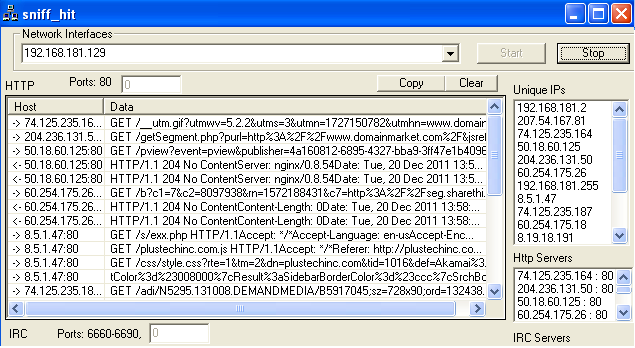
\includegraphics[width=1\textwidth]{graph/SysAnalyser.png}
\caption{SysAnalyser tool for dynamic analysis.}
\label{fig:SysAnalyser}
\end{figure}

The advantage of Dynamic malware technique is simple. The process of malware analysis is running malware and making sure what will happen in 
system.

However, there are some disadvantage of dynamic malware analysis technique. These dynamic techniques are vulnerable to a variety of anti-monitoring defenses such as \emph{time bombs} and \emph{logic bombs}. Additionally, these techniques can be slow and tedious to identify and disable. In addition, a dynamic analysis may fail to identify the malware if the behavior of malware is not logged during the analysis process. Furthermore, Much time is required to prepare environment for malware analysis, such as virtual machine environment or sandbox. Moreover, Some malware cannot be executed in virtual machine environment. In conclusion, dynamic technique is not enough for malware analysis. 

\subsection{Static malware analysis}

Static malware analysis is technique that identifies malware program without executing it. With the static malware analysis technique, researcher performs reverse engineering using disassemble tools, decompile tools, source code analyzer tools such as IDA pro and Ollydbg in order to understand malware by seeing the structure of malware. Static malware analysis has an advantage that it can completely discover the purpose and functionality of malware. However, research needs time to understand the malware functionality by analysing malware structure.

In addition, most modern malwares use packer to modify itself. Packer is a program that modify other program files to compress their content. When a packer compress, encrypts, otherwise modifies an executable program, the program looks much different before it was packed. For analysing malware by Ollydbg or IDA pro, malware must be unpacked. PEid is a program that can find the signature of a known compiler or packer. Figure \ref{fig:PEid} shows PEiD is applied to identify identifies the compiler and packer used by the malware author.

\begin{figure}[h!]
\centering
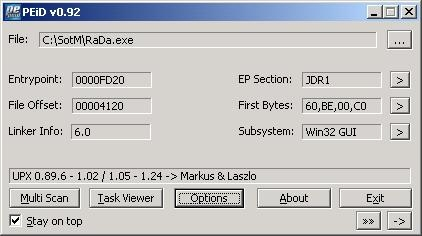
\includegraphics[width=1\textwidth]{graph/PEid.jpg}
\caption{PEid identify the packer used by the malware author.}
\label{fig:PEid}
\end{figure}

Figure \ref{fig:OllyDbg} shows the example of using OllyDbg tool in order to analyse malware. 


\begin{figure}[h!]
\centering
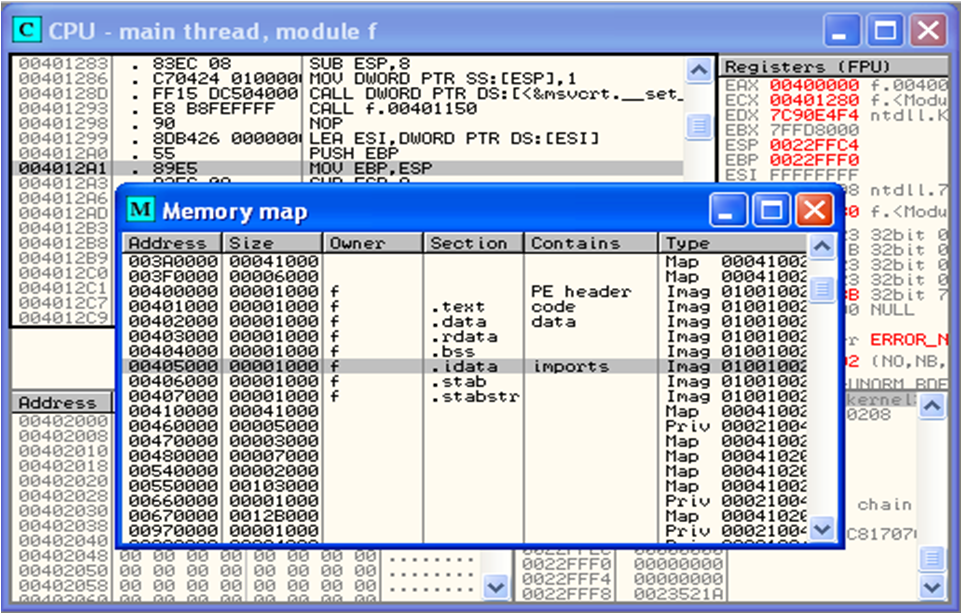
\includegraphics[width=1\textwidth]{graph/OllyDbg.png}
\caption{Ollydbg tool for static analysis.}
\label{fig:OllyDbg}
\end{figure}
Figure \ref{fig:IDApro} shows the example of using IDA pro tool in order to analyse malware. 

\begin{figure}[h!]
\centering
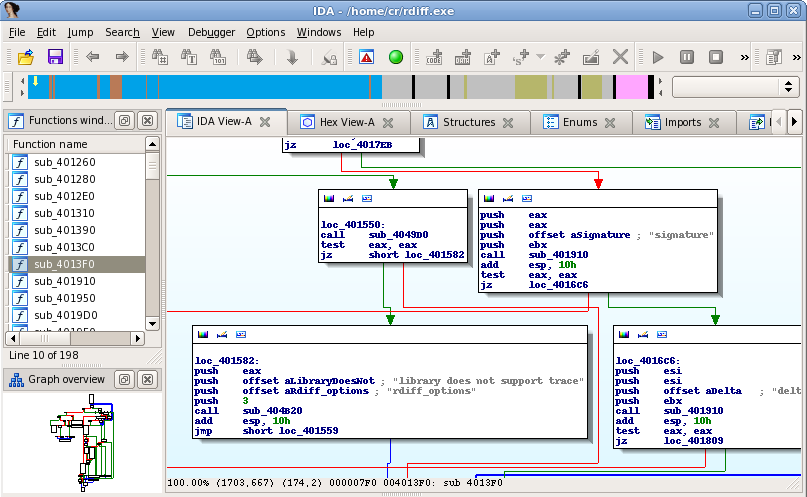
\includegraphics[width=1\textwidth]{graph/idapro.png}
\caption{IDA pro tool for static analysis.}
\label{fig:IDApro}
\end{figure}
\section{Malware categories}

In general, malware is classified into a few categories or types based on behaviors, method of infection, and the resulting propagation of malware. For example, this is some malware categories: virus, trojan, worm, spyware, and rookit. The categories detail specific types of malware threats:

\begin{itemize}
\item Virus :"Software which infects other application and use them as a spreading medium"\cite{BlackHat}.
\item Trojan :"A malicious application which present itself as something else"\cite{BlackHat}.
\item Worm :"Code with ability to spread from computer to computer by means of different network protocols"\cite{BlackHat}.
\item Spyware :"Application aiming to havest personal information"\cite{BlackHat}.
\item Rookit :"Hidden tools providing stealth services to its writer"\cite{BlackHat}.
\end{itemize}

However, As the different between the categories are a bit fuzzy, and the classes are obviously not exclusive. In addition, depend on purpose of virus industry a unique malware can belong to rookit, virus, or spyware. The detail of malware categories is presented on the next section. 
\subsection{Use virus total to detect the name of categories.}

In this thesis, MD5 hash is used to detect malware name which provided by many anti-virus vendor. An MD5 hash is generated by MD5 Message-Digest Algorithm, is a widely used cryptographic hash function that produces a 128-bit (16-byte) hash value. An MD5 hash is typically expressed as a 32-digit hexadecimal number, and MD5 is not collision resistant\cite{wiki1}.

\subsection{Using virus total to getting vendor name}
In this paper, MD5 hash of malware is used to search the name of malware by virus total. Virustotal is a web service that analyzes malware files and facilitates quick detection of viruses, worms, trojans, and all kinds of malware detected by antivirus engines. Malware's name is provided by various anti-virus vendor, but there are many name for unique malware. The Figure \ref{fig:virustotal_listname} shows malware name detected by antivirus engines. 
\begin{figure}[h!]
\centering
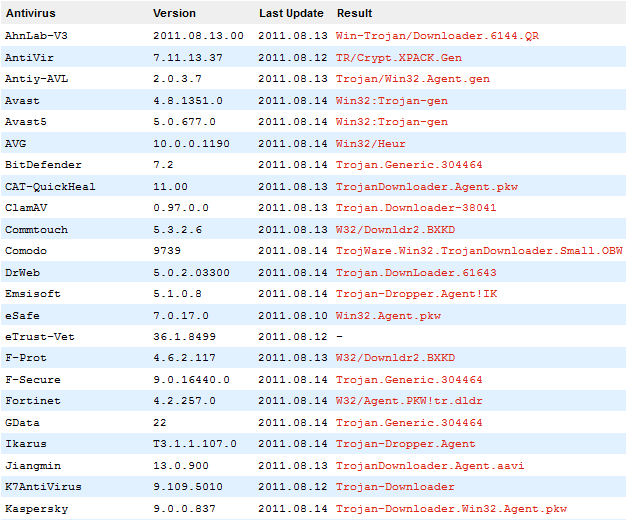
\includegraphics[width=1.0\textwidth]{graph/virustotal_listname.png}
\caption{Malware name is detected by antivirus engines.}
\label{fig:virustotal_listname}
\end{figure}
\section{Problems of malware name} 
As the malware name detected by anti-virus engines show in Figure \ref{fig:virustotal_listname}, unique malware is not classified into unique name. For each anti-virus vendor, the name of malware detected is different to the other anti-virus vendor. The classification of each anti-virus engine is unlike others. Therefore, malware detected by anti-virus engines cannot provide meaningful characterization of malware for virus researcher. In order to overcome this problem, this paper proposed to classify the malware into families based on malware specific target and its operation behavior. 
As a result of malware name detected by anti-virus vendor was presented above, the new malware families is required for detect meaningful characterization of malware. 
\section{Malware families is used in this paper} 
This paper use malware families which is reported by Information-technology Promotion Agency \cite{ipa}. The table show malware families used in this paper such as Win32/Virut, Win32/Autorun, Win32/IRCbot, Win32/Gaobot, Win32/Waledac, Win32/Downadup, Win32/Sality, and W32.Mota.

\begin{center}
\begin{table}
\begin{tabular}{ l | p{13cm} }
Malware familes & Summary\\ \hline
Win32/Virut & "Win32/Virut is a family of file infecting viruses that target and infect .EXE and .SCR files accessed on infected systems.
 Win32/Virut also opens a backdoor by connecting to an IRC server, allowing a remote attacker to download and run files on the infected computer." \cite{virut}\\ \hline
Win32/Autorun & "Win32/Autorun is a family of worms that spreads by copying itself to the mapped drives of an infected computer. The mapped drives may include network or removable drives." \cite{autorun}\\\hline
Win32/IRCbot & "Win32/IRCbot is a large family of backdoor Trojans that targets computers running Microsoft Windows. The Trojan drops other malicious software and opens a backdoor on the infected computer to connect to IRC servers. The Trojan can maintain multiple IRC server connections simultaneously to receive commands from attackers." \cite{ircbot}\\ \hline
Win32/Gaobot & "The Win32/Gaobot worm family spreads using different methods, depending on the variant. Some variants spread to machines with weak passwords. Others exploit vulnerabilities to infect machines. Once a machine is infected, the worm connects to an IRC server to receive commands." \cite{gaobot}\\ \hline
Win32/Waledac & "Win32/Waledac is a trojan that is used to send spam. It also has the ability to download and execute arbitrary files, harvest email addresses from the local machine, perform denial of service attacks, proxy network traffic and sniff passwords." \cite{walemac}\\ \hline
Win32/Downadup & "Win32/Downadup attempts to spread to network shares by brute-forcing commonly used network passwords and by copying itself to removable drives." \cite{downadup}\\ \hline 
Win32/Sality & "Virus:Win32/Sality is a family of polymorphic file infectors that target Windows executable files with the extensions .SCR or .EXE. They may execute a damaging payload that deletes files with certain extensions and terminates security-related processes and services.\\ \hline 
W32.Mota & W32.Mota is a worm that propagates by sending itself to email addresses gathered from the computer." \cite{mota}\\ \hline 
\end{tabular}
\caption{Malware}
\label{tab:malwarefamilies}
\end{table}
\end{center}


\chapter{Related research}\label{chap:3}
%THE SYSTEM ARCHITECTURE
%
%
This chapter presents the recent approach for automatically classify malware into malware families. For the reason that the detection based static signature is no longer effective in chapter \ref{chap:2}, at this time new malware classification method is required to detect mawlare writers used avoidance technique.

\section{Flow graph}
An another approach is using emulator to automatically unpack the packing malware, then from reverse code produce flowgraph, then flowgraph matching to perform classification\cite{silvio}. The system created by the approach follows:

\begin{itemize}
\item Fist, System automatically unpack malware based on application level emulation, and then use entropy analysis to detect.
\item Second, Produce control followgraph by using graph invaiant based signature in order to measure similarity between malware.
\item Next, Generic string based control flow signature, in order to using string edit distancce. Automatically unpack malware based on application level emulation.
\item Finally, Malware classification use a set similarity function and a set similarity search algorithm to represent benign and malicious classes.
\end{itemize}

The disadvantage in flowgraph approach is high cost of runtime complexity. Firstly, runtime complexity of of malware classification is $O(N\log{M})$ where M is the number of control follow graphs in database, and N is the number of control follow graph input binary \cite{silvio}. In addition, To identify two flowgraph is $N^{3}$, and N is the number of nodes in each graph. Further more, needs to unpack the sample if it was packed with an executable packer. There fore, this approach is ineffective in malware classification system with a large number of instances.

In addition, malware classification based flowgraph approach cannot accurately detect metamorphic malware. As presented at chapter \ref{chap:2}, metamorphic malware can recode it self with program follow modification, function reordering. There fore, it is hard to classify malware based a set  similarity between follow graph.
\section{Optimizing decision tree in malware classification system by using Generic Algorithm}
In this time, malware classification system can use machine learning classifier. The main idea of machine learning technique classifier is search algorithm that learn from externally supplied instances to produce a concise model of the distribution, which then  make prediction about new  instances. Current machine learning classifier in malware classification include: Naive Bayse, Suport Vector machine, Decision tree, K-nearest Neighbor \cite{mohd}. This approach use combining Generic algorithms with Decision tree. The data set is separated in training data set and testing data set. The data set is include:

// Malware target, specific target for malware attack\\
vector<list<MalwareClass\*>> \_slots;\\
// Malware classes for chromosome\\
hash\_map<MalwareClass\*,int> \_Dataclasses;\\
hash\_map<MalwareClass\*,int> \_Appsclasses;\\
hash\_map<MalwareClass\*,int> \_Sysclasses;\\
hash\_map<MalwareClass\*,int> \_Dosclasses;\\

Generic algorithm is methods that analogous to the process of natural evolution. Generic algorithm is used to optimize decision tree in order to accurately classify malware. Malware classification system, which implemented by the combining generic algorithm with decision tree algorithm approach, is for classify malware into two classes: benign program and malicious program, not for detect semantic characterization of malware by classifying malware into families. There fore, the combining generic algorithm with decision tree algorithm approach cannot use for detecting semantic characterization of malware.
\section{Conclustion}
To achieve fast malware classification, two approach is described before can not be used in this system. New approach for fast malware classification system will introduced in the next chapter. 
\chapter{Classification based on malware's meta-data using decision tree approach}\label{chap:4}
%EXPERIMENTAL RESULTS AND ANALYSIS
%
%
This chapter describes Win32 executive files structure, known as PE files structure, that is used in classification system as malware meta-data. Afterwards, the machine learning technique called decision tree method is mentioned in classification malware system. Finally, we will propose the classification approach based on malware's meta-data using decision tree technique. 

\section{PE file format\cite{peheaderci}}
\subsection{The PE File Format}

The Portable Executable (PE) file format has been designed for use by all Win32 based system. The general layout of a PE file is given in Figure \ref{fig:pefiles} . PE header consists of four parts: a MS-DOS session including DosMZ header and Dos stub; PE header; a section table; and images pages consisting of several different regions such as .text session, and .data session.
\begin{figure}[h!]
\centering
\includegraphics[width=1\textwidth]{graph/pefiles.png}
\caption{The general layout of a PE file.}
\label{fig:pefiles}
\end{figure}

The PE file format starts with DOS MZ header. The first two bytes - "MZ" of the header is the DOS EXE signature. The first few hundred bytes of the typical PE file are taken up by the MS-DOS stub. This stub is a tiny program that displays a string as "This program cannot be run in MS-DOS mode.". 

The following part is PE header. The fields of this structure contain only the most basic information about the file such as the locations and sizes of the code and the data areas. These data structures of PE header will be explained shortly.

Following the PE header is the session table. The section table is an array of IMAGE\_SECTION\_HEADERs structures. An IMAGE\_SECTION\_HEADER provides information about its associated section such as location, length, and characteristics. The number of elements in this array is given in the PE header, known as \emph{NumberOfSections} field. There are commonly at least two sections in a PE file: code and data. Figure \ref{fig:pefiles1} shows a section table for a typical PE file.

\begin{figure}[h!]
\centering
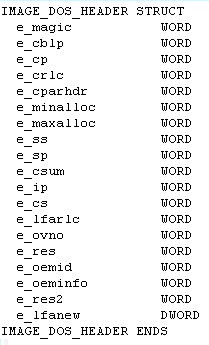
\includegraphics[width=0.8\textwidth]{graph/dosHeaderStructure.png}
\caption{A section table for a typical PE file.}
\label{fig:pefiles1}
\end{figure}

That is all about the physical layout of the PE file format. The major steps in loading a PE file into memory are described as follows:

\begin{itemize}
\item When the PE file is running, the PE loader examines the DOS MZ header for the offset of the PE header. If it is found, it would skip to the PE header.
\item The PE loader checks if the PE header is valid. Then, it goes to the end of the PE header if the PE header is valid.
\item Following the PE header is the section table. The PE header reads information about the sections and maps those sections into memory using the file mapping.
\item After the PE file is mapped into memory, the PE loader concerns itself with the logical parts of the PE file, such as the import table.
\end{itemize}
\begin{figure}[h!]
\centering
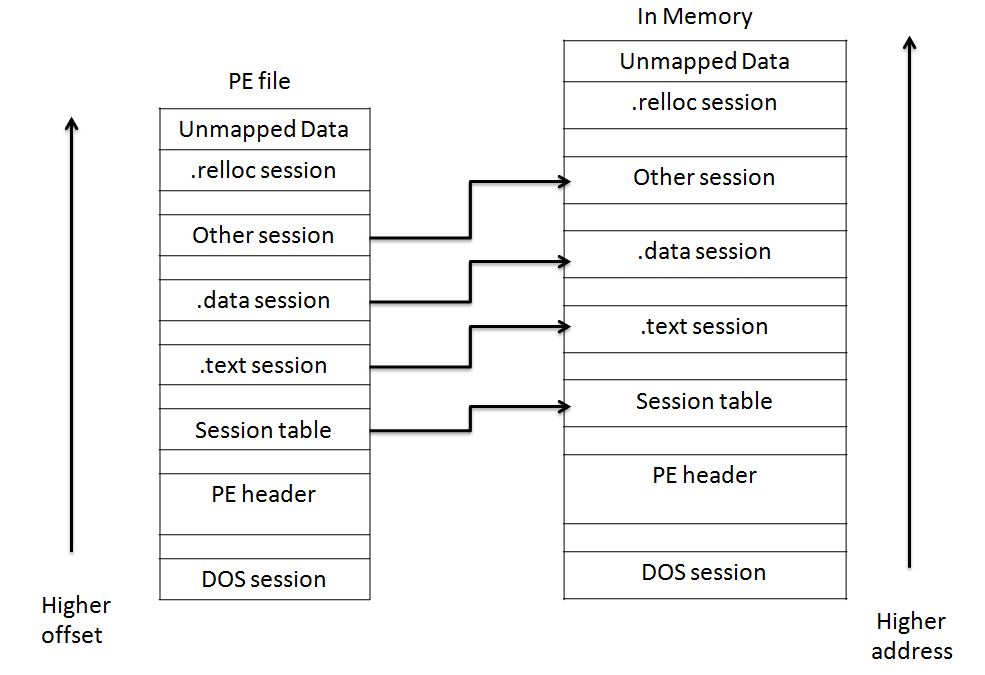
\includegraphics[width=1\textwidth]{graph/pe1.png}
\caption{PE file format.}
\label{fig:pe1}
\end{figure}


\subsection{The PE Header}


\begin{figure}[httb]
\centering
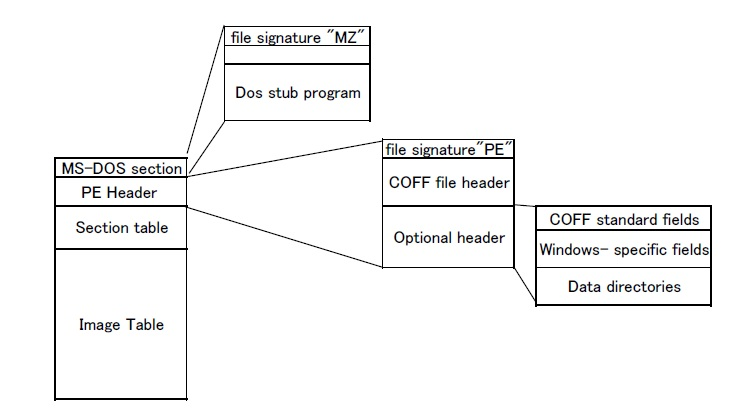
\includegraphics[width=1\textwidth]{graph/peheader1.jpg}
\caption{Layout a file in the PE header format.}
\label{fig:peheader}
\end{figure}
The PE header is the second part of the PE files structure. The PE header starts with two characters "PE" known the PE header file signature. The main PE header is a structure of type IMAGE\_NT\_HEADERS, which is defined in WINNT.H. The structure of PE header consists of a DWORD and two substructures composed of FileHeader and OptionalHeader. IMAGE\_NT\_HEADERS contains the following three fields:
\begin{verbatim}
DWORD Signature;
IMAGE_FILE_HEADER FileHeader;
IMAGE_OPTIONAL_HEADER OptionalHeader;
\end{verbatim}
Following the PE signature DWORD in the PE header is a structure of type IMAGE\_FILE\_HEADER. 
\begin{verbatim}
typedef struct _IMAGE_FILE_HEADER {
  WORD  Machine;
  WORD  NumberOfSections;
  DWORD TimeDateStamp;
  DWORD PointerToSymbolTable;
  DWORD NumberOfSymbols;
  WORD  SizeOfOptionalHeader;
  WORD  Characteristics;
} IMAGE_FILE_HEADER, *PIMAGE_FILE_HEADER;
\end{verbatim}
The fields of this structure contain only the most basic information about the file. The fields of the IMAGE\_FILE\_HEADER include:
\begin{itemize}
\item Machine: The CPU that this file is intended for.
\item NumberOfSections: The number of the members in section
\item TimeDateStamp: The time that the linker
\item PointerToSymbolTable: The file offset of the COFF symbol table. 
\item NumberOfSymbols: The number of symbols in the COFF symbol table.
\item SizeOfOptionalHeader: The size of an optional header that can follow this structure.
\item Characteristics: The size of an optional header can follow this structure. If there are no relocations in this file, characteristics will be 0x0001. Otherwise, the file is an executable image, characteristics will be 0x0002.  If file is a dynamic-link library, not a program, characteristics will be 0x2000.
\end{itemize}

Following the file header is the optional header which consists of three parts: COFF standard fields, Windows specific fields, and data directories. The first part includes the COFF standard field which contains the sizes of various parts of code, and the \emph{AddressOfEntryPoint} which indicates the location of the entry point of the application and the location of the end of the Import Address Table(IAT). Then, the second part contains the information of OS. Finally, the Data directories field contains the information of Session table.

The following is the structure of optional header. 
\begin{verbatim}
typedef struct _IMAGE_OPTIONAL_HEADER {
  WORD                 Magic;
  BYTE                 MajorLinkerVersion;
  BYTE                 MinorLinkerVersion;
  DWORD                SizeOfCode;
  DWORD                SizeOfInitializedData;
  DWORD                SizeOfUninitializedData;
  DWORD                AddressOfEntryPoint;
  DWORD                BaseOfCode;
  DWORD                BaseOfData;
  DWORD                ImageBase;
  DWORD                SectionAlignment;
  DWORD                FileAlignment;
  WORD                 MajorOperatingSystemVersion;
  WORD                 MinorOperatingSystemVersion;
  WORD                 MajorImageVersion;
  WORD                 MinorImageVersion;
  WORD                 MajorSubsystemVersion;
  WORD                 MinorSubsystemVersion;
  DWORD                Win32VersionValue;
  DWORD                SizeOfImage;
  DWORD                SizeOfHeaders;
  DWORD                CheckSum;
  WORD                 Subsystem;
  WORD                 DllCharacteristics;
  DWORD                SizeOfStackReserve;
  DWORD                SizeOfStackCommit;
  DWORD                SizeOfHeapReserve;
  DWORD                SizeOfHeapCommit;
  DWORD                LoaderFlags;
  DWORD                NumberOfRvaAndSizes;
  IMAGE_DATA_DIRECTORY DataDirectory[IMAGE_NUMBEROF_DIRECTORY_ENTRIES];
} IMAGE_OPTIONAL_HEADER, *PIMAGE_OPTIONAL_HEADER;
\end{verbatim}

The fields of Optional header are described as follow: 
\begin{itemize}
\item Magic: appears to be set to 0x010B.
\item MajorLinkerVersion
\item MinorLinkerVersion: the version of the linker that produced this file.
\item SizeOfCode: this field matches the size of the .text section.
\item SizeOfInitializedData: 
\item SizeOfUninitializedData: 
\item AddressOfEntryPoint: 
\item BaseOfCode: 
\item BaseOfData: 
\item ImageBase: 
\item SectionAlignment: 
\item FileAlignment: 
\item MajorOperatingSystemVersion: 
\item MinorOperatingSystemVersion: 
\item MajorImageVersion: 
\item MinorImageVersion: 
\item MajorSubsystemVersion: 
\item MinorSubsystemVersion: 
\item Reserved1: 
\item SizeOfImage: 
\item SizeOfHeaders: 
\item CheckSum: 
\item Subsystem: 
\item DllCharacteristics: 
\item SizeOfStackReserve:
\item SizeOfStackCommit: 
\item SizeOfHeapReserve:
\item SizeOfHeapCommit: 
\item LoaderFlags: 
\item NumberOfRvaAndSizes:
\item DataDirectory:
\end{itemize}

\section{Decision tree\cite{decisiontree}}

Decision tree is a machine learning technique for building knowledge-based systems by inductive inference from examples. Decision tree is to create a model that predicts the value of a target variable based on several input variables. An example is shown on the Figure \ref{fig:decisiontreesample} from the data Table \ref{fig:decisiontreesampletable}. The decision tree is created the Table from Each interior node corresponds to one of the input variables. There are edges to children for each of the possible values of that input variable. Each leaf shows a value of the target variable.
\begin{figure}[h!]
  \begin{center}
    \begin{tabular}{ | l | l | l | l | l }
     \hline
    Condition & Class & Attribute 1 &  Attribute \\ \hline
    1 & A & 0 & 0 & ... \\ 
	2 & B & 1 & 0 & ... \\ 
	3 & C & 1 & 1 & ... \\ 
	... & ... & ... & ... & ... \\ 


    \end{tabular}
	\end{center}
     \caption{The data table.}
    \label{fig:decisiontreesampletable}
\end{figure} 
\begin{figure}[httb]
\centering
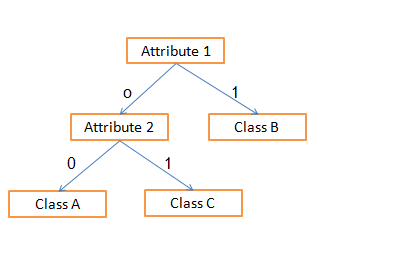
\includegraphics[width=1\textwidth]{graph/decisiontreesample.png}
\caption{Decision tree sample.}
\label{fig:decisiontreesample}
\end{figure}

In data mining, the decision tree technique can be described also as the combination of mathematical and computational techniques to aid the description, categorization and generalization of a given set of data.

Data comes in records of the form
\begin{equation}
    (x,Y) = (x_1, x_2, x_3, ..., x_k, Y) 
\end{equation}

The dependent variable, $Y$ which is the target variable is analysed to understand, classify or generalise. The vector x is composed of the input variables, $x_{1}, x_{2}, x_{3}$ that are used for that task.
\section{Classification based on malware's meta-data using decision tree approach}

To make malware classification rapid and correct, decision tree algorithm is used in malware classification system.

As the previous section, data comes in records of the form:\begin{equation}
    (x,Y) = (x_1, x_2, x_3, ..., x_k, Y) 
\end{equation}

In malware classification system, Y is malware families name, $x_{1}, x_{2}$,...,$x_{3}$ is malware file's meta-data. Malware name is provided by anti-virus engines that presented in chapter \ref{chap:2} cannot used in this system. The new malware families is required for detect meaningful characterization of malware. This classification system use famous malware families reported in Information technology agency such as netsky, mydoom, autorun, mytob, and other famous malware families. Therefore, when new malware is classified into famous malware families, researcher detect some meaningful characterize of malware, and reduce time for malware analysis. 
\section{Conclusion}
In this chapter, our approach is proposed with the technique used in malware classification system.
In the next chapter, propose the system design and implementation will be proposed.
\chapter{Implementation}\label{chap:5}
In this chapter, the work of implementing malware classification system will be described. Starting with the implementing environment, this chapter will go through introduction of the meta-data used in
this system, and finally system software implementation which is written in PHP language.
%EXPERIMENTAL RESULTS AND ANALYSIS
%
%
\section{Environment}

In proposing system, operator system, Database, and are all operated in one computer. Technical information of employed computer is shown as in Table \ref{table:environment}. DecisionTree $1.5$ is good choice to this implementation, with these following reasons:
\begin{itemize}
\item The library constructs a decision tree from multidimensional training data.
\item The library use the decision tree thus constructed for classifying unlabeled data. \cite{decisiontreelibrary}.
\end{itemize} 
  \begin{table}
\begin{center}  
\label{table:environment}
    \begin{tabular}{ | l | l | l | }
     \hline
    Element &  Attribute  &  Environment \\ \hline
    OS & Computer & Ubuntu 11.04 \\ \hline
	Database & Mysql & Mysql 5.0 \\ \hline
	Programming language & C & gcc  \\ \hline
	 & PHP & PHP 5.0  \\ \hline
	 & Python & Python 2.7 \\ \hline
	 Library & DecisionTree 1.5 &  ID3 \\ \hline
    \end{tabular}
    \caption{Implementation environment of the malware classification system.}  
    \end{center}
  \end{table}
  
\section{Overview}
The system uses machine learning technique, named decision tree algorithm for malware classification. The goal is classifying malware fast and decision tree algorithm is used to achieve. Classification is a form of supervised learning, which requires training data, with known input/output, to form knowledge \cite{tonylee}. As mentioned in Figure \ref{fig:system_architec}, the system contains three following parts.

\begin{itemize}
\item First part: Read binary file to take meta data and input to database.
\item Second part: Manually cluster malware loaded from database.
\item Third part: Use decision tree algorithm to classify malware.
\end{itemize}
\begin{figure}[h!]
\centering
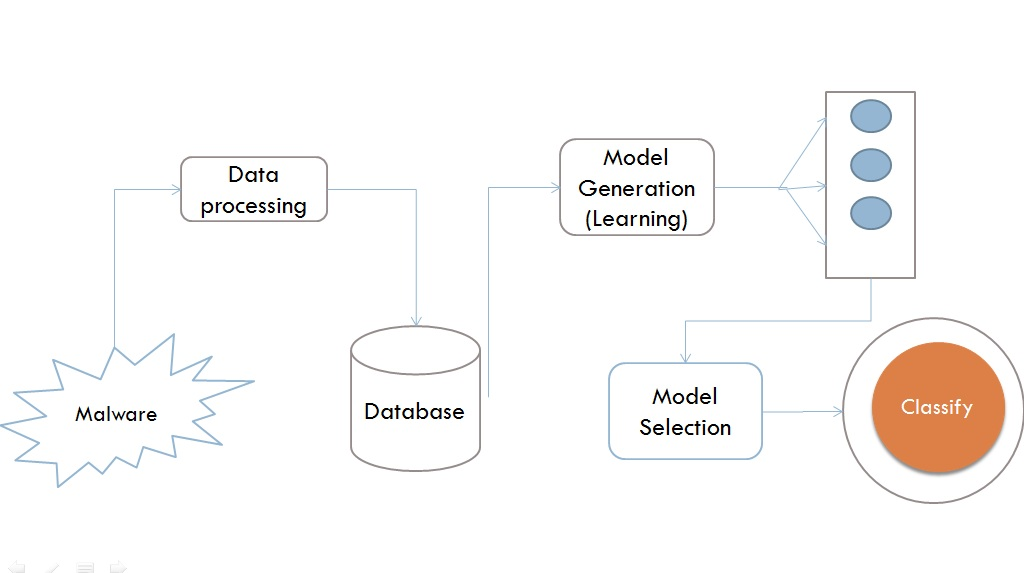
\includegraphics[width=1\textwidth]
{graph/system_architec.jpg}
\caption{The system architecture.}
\label{fig:system_architec}
\end{figure}

A vast amount of malware need analyzing, and the system uses database to store malware file's meta-data, to easily control a large number of data and to share them in the internet among web browsers.
The flow of data is shown in the Figure \ref{fig:system_architec}. At first, binary file meta-data are read, and all of the meta-data are input into database. In the second part, the system exports meta-data in database as the training data to create the decision tree for classifying malware. Finally, the decision tree algorithm created in the second step is utilized to class  unknown malware into the different malware families. 
%CLASSFICATION BASE ON DECISION TREE
%
%
\section{Classification based on machine learning technique} 
\subsection{Meta-data}
Meta-data is simply data about data. The malware file's meta-datas are all simply information about malware file. PE header includes meta-data of MS-DOS section; COFF file header; Optional header; Section header; and other types of data in sections include API import and export table. Meta-datas are many data about malware. The classification system based on can identify malware changed malware signature and syntax by using code reordering, code rewriting, and instruction insertion. Additionally, malware's meta-data can be easy received. 
Therefore, in order to create a fast and accuracy malware classification system, the system only uses PE header's meta-data to classify malware.
 
There is a problem that PE file's meta data value is too large to detect unknown malwares which have meta-data's differences from the training data of the system. The meta-data of PE header file are separated  to give semantic information for malware classification. For example, normally \emph{ImageBase} field of PE header file has value of 400000h \cite{goppit}. In this system, the meta-data of PE header file is separated into $7$ class by this calculation:
\begin{equation}
SemanticMetaData = MetaData \bmod 7
\end{equation} 

Decision tree modeling predicts effects $7$ is larger enough to separate malware file's meta-data value into classes. Additionally, $7$ is a prime number so that it is better to divide malware file's meta-data value into $7$ classes than another number. For example, The \emph{MajorLinkerVersion} field in PE file has a list of values as: $0x00003000$, $0x00001000$, and $0x00006000$. By the above equation, the semantic value of these value is as follows: 3,1,6. However, if the system use $8$, the semantic value of these value are as follows: 0. In conclusion, $7$ is good choice to separate malware file's meta-data value.

\subsection{Create training data}

In this system use decision tree technique. The attributes of decision tree described in previous subsection. We mentions the method to identify malware family name based on malware name provided by anti-virus vendors.

Virustotal is a service that analyzes malware and facilitates quick collection of viruses, worms, trojans, and all kinds of malware are detected by antivirus vendor such as Norton and Kaspersky \cite{virustotal}. This research applies virustotal service to take the name of malware provided by the vendors and uses it to cluster malware into malware families with semantic information.

Figure \ref{fig:clustering} indicates http post technique to automatically get name from virus total service and cluster malware into malware families which given in Figure \ref{fig:familymalware}.

Malware families in this classification system are as follows: Win32/Virut, Win32/Autorun, Win32/IRCbot, Win32/Gaobot, Win32/Waledac, Win32/Downadup, Win32/Sality, and W32.Mota. 

The disadvantage of using Virustotal to identify malware's families that a unique malware has many different names provided by many antis-virus vendors. Therefore, if unique malware has two or more families name provided by anti-virus vendor, unique malware will be classed into the most reported malware family.
 
\begin{figure}[h!]
\centering
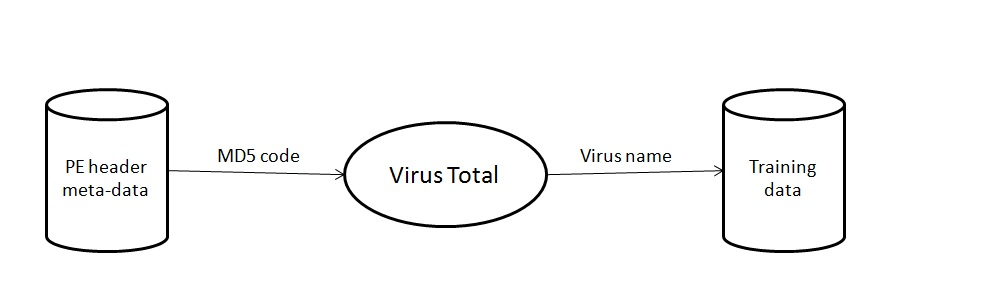
\includegraphics[width=1\textwidth]{graph/clustering.jpg}
\caption{Clustering method.}
\label{fig:clustering}
\end{figure}

\subsection{Classification}
\begin{figure}[h!]
\centering
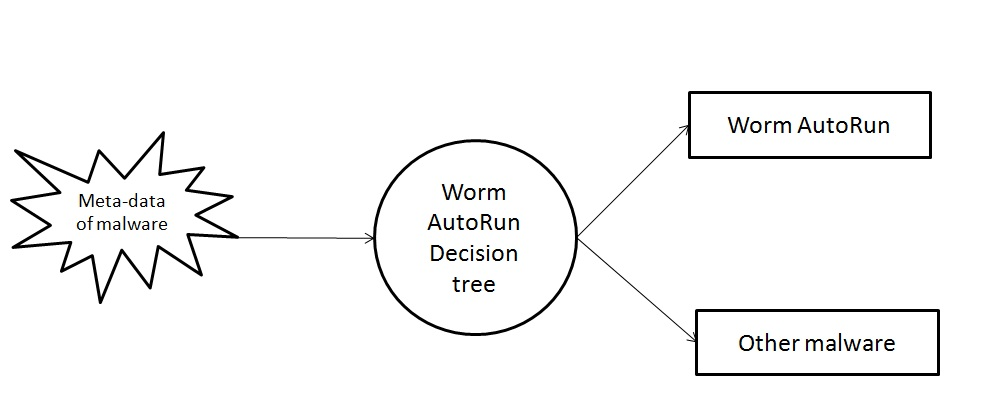
\includegraphics[width=1\textwidth]{graph/classificationdecision.jpg}
\caption{Worm autorun decision tree.}
\label{fig:classificationdecision}
\end{figure}

To make malware classification rapid and correct, decision tree algorithm is utilized. At that time, it is easy to update a new malware family, the classification uses decision tree algorithm to determine each malware family. For example, based on training data from clustering part, six decision trees are created. The worm autorun decision tree is indicated in Figure \ref{fig:classificationdecision}.

Malware' meta-data are known as input data for each decision tree, and the decision tree determines whether the malware is of worm autorun family or not. If the input malware belongs to worm autorun, malware classification shall detect which the family that malware is, otherwise it moves to the next decision tree. Lists of malware PE header file's meta-data are Magic, MajorLinkerVersion, MinorLinkerVersion, SizeOfCode, SizeOfInitializedData, SizeOfUninitializedData, AddressOfEntryPoint, BaseOfCode, BaseOfData, ImageBase, SectionAlignment, FileAlignment, MajorOperatingSystemVersion, MinorOperatingSystemVersion, MajorImageVersion, MinorImageVersion, MajorSubsystemVersion, MinorSubsystemVersion, Reserved1, SizeOfImage, SizeOfHeaders, CheckSum, Subsystem, DllCharacteristics, SizeOfStackReserve, SizeOfStackCommit, SizeOfHeapReserve, SizeOfHeapCommit, LoaderFlags, NumberOfRvaAndSizes, Machine, NumberOfSections, TimeDateStamp, PointerToSymbolTable, NumberOfSymbols, SizeOfOptionalHeader, Characteristics. The value of each field in PE header has semantics for decision tree algorithm if it is appeared at 10\% in malware training data. With this approach, the semantic value list of meta-data malware is made. For example, this is a list of meta-data created :1, 2, 6, 4, 0, 1, 1, 4, 0, 200, 4, 0, 0, 0, 4, 0, 0, 1.00E+00, 200, 0, 2, 0, 100000, 4000, 100000, 1000, 0, 10, 14c, 2, 1000, 8, 0, e0, 3, 818e. This is value before being computed :35328, 10b, 2, 0, 6200, 0, 200, b32e, b000, 9000, 400000, 1000, 200, 3, 0, 0, 0, 4, 0, 0, d000, 400, afe8, 2, 0, 1000, 1000, 10000, 0, 0, 10, 14c, 6, 0, 0, 0, e0, 10e. 
The malware classification part is shown in Figure \ref{fig:classification}. The training data from the malware clustering part is used to create the order of decision tree that makes malware classification system correct.
The decision tree is given as in Figure \ref{fig:decisiontreeworm}. When PE header's meta-data of malware is inputted into the worn autorun decision tree for determining unknown malware. Then, it decides whether it belongs to worm auto run family or not.
\begin{figure}[h!]
\centering
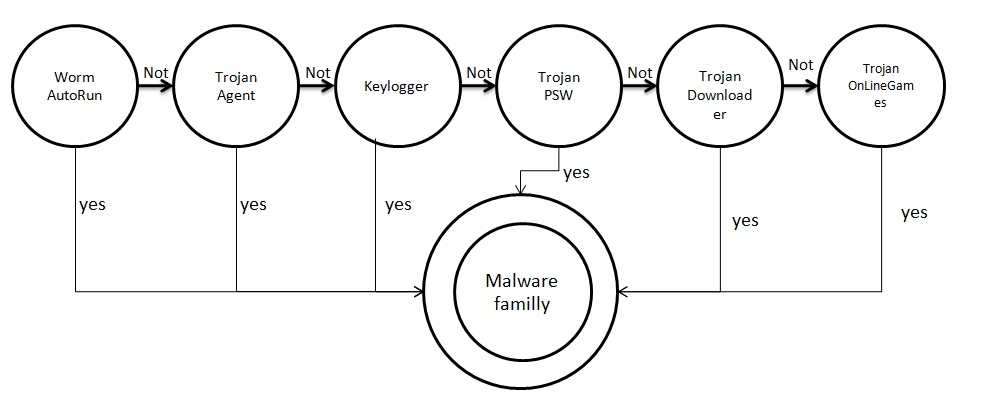
\includegraphics[width=1\textwidth]{graph/classification.jpg}
\caption{Malware classification system.}
\label{fig:classification}
\end{figure}
\begin{figure}[h!]
\centering
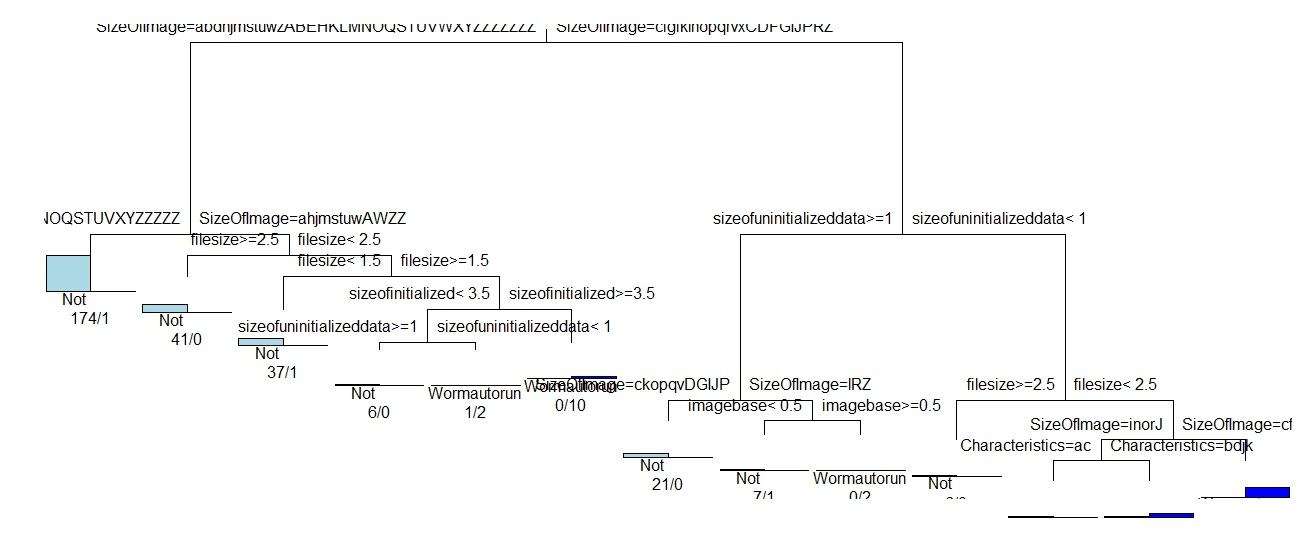
\includegraphics[width=1\textwidth]{graph/decisiontreeworm.jpg}
\caption{Worm autorun decision tree.}
\label{fig:decisiontreeworm}
\end{figure}

\chapter{Evaluation}\label{chap:6}


\section{Accuracy evaluation}

In 4436 malwares obtained, 4181 of them are to construct a decision trees. The number of each malware families is shown in Table \ref{table:trainingdata}. Then, 255 remaining malwares meta-data are kept to test experimental result the system.
\begin{table}
  \begin{center}
    \begin{tabular}{ | l | l |}
     \hline
    Malware & Number\\ \hline
    Virut & 2243\\ \hline
	IRCbot & 1169\\ \hline
	Gaobot  & 265\\ \hline
	Autorun & 195\\ \hline
	Downadup &  103\\ \hline
	Mota & 79\\ \hline
	Sality  & 66  \\ \hline
	WaledacMota & 61\\ \hline
    \end{tabular}
	\end{center}
     \caption{Training data.}
      \label{table:trainingdata}
\end{table}

In the decision tree, 255 malwares are chosen to check the experimental result of system. 

 The number of each malware families is shown in Table \ref{table:testdata}
 \begin{table}
  \begin{center}
    \begin{tabular}{ | l | l |}
     \hline
    Malware & Number\\ \hline
    Virut & 200\\ \hline
	IRCbot & 100\\ \hline
	Gaobot  & 20\\ \hline
	Autorun & 10\\ \hline
	Downadup &  10\\ \hline
	Mota & 5\\ \hline
	Sality  & 5  \\ \hline
	WaledacMota & 5\\ \hline
    \end{tabular}
	\end{center}
     \caption{Test data.}
      \label{table:testdata}
\end{table}
Table \ref{table:experimentalresult} reveals that result. Some of the data in axis show these total number of malware in that family, and that number is separated into groups that these malwares has been classified by the system. For example, there are four malwares in Win32/Virut family, and three of them are successfully sorted into Win32/Virut family and, while one malware is in other family. Therefore, the system recognizes the trojan agent family with 75 \% of accuracy.
\begin{table}
  \begin{center}
    \begin{tabular}{ | l | l | l | l | l | l | l | l | l | l |}
     \hline
    Malware & Virut & IRCbot& Gaobot &  Autorun & Downadup  & Mota & Sality & Waledac & Accuracy\\ \hline
    Virut & 98 & 102 & 0 & 0 & 0 & 0  & 0  & 0 & 49\%\\ \hline
    IRCbot & 5 & 95 & 0 & 0 & 0 & 0  & 0  & 0 & 95\%\\ \hline    
	Gaobot & 0 & 20 & 0 & 0 & 0 & 0  & 0  & 0 & 0\%\\ \hline
	Autorun & 10 & 10 & 0 & 0 & 0 & 0  & 0  & 0 & 0\%\\ \hline	
	Downadup & 0 & 1 & 0 & 9 & 0 & 0  & 0  & 0 & 90\%\\ \hline
	Mota  & 2 & 3 & 50 & 0 & 0 & 0  & 0  & 0 & 0\%\\ \hline
	Sality  & 1 & 1 & 50 & 0 & 1 & 2  & 0  & 0 & 40\%\\ \hline	
	Waledac & 2 & 3 & 50 & 0 & 0 & 0  & 0  & 0 & 0\% \\ \hline
    \end{tabular}
	\end{center}
     \caption{Experimental result}
    \label{table:experimentalresult}
\end{table}
The accuracy of this classification system:
\begin{equation}
Accuracy=\frac{98+95+9+2}{355}=57\%
\end{equation}

The other classification is often classify malware into benign and malicious software. The system implemented in this thesis classify malware into the malware family. Therefore, system The system is useful to help virus researcher determine the malware family that unknown malware belongs to. The malware family contains Win32/Virut, Win32/Autorun, Win32/IRCbot, Win32/Gaobot, Win32/Waledac, Win32/Downadup, Win32/Sality, W32.Mota, known as famous malware family. Virus researchers who know the family of malware can easily find out some semantic similarities between malwares and shows their inner similarity in behavior and static malware characteristics.

\section{Efficiency  of classification}
The evaluation was performed on a 2.4 HZ core i3 laptop with 4G memory, running in ubuntu 11.4. 	

To evaluate the speed of the malware classification system, 2999 malware samples were evaluate the classification efficiency of the system.
Figure \ref{fig:evaluation} show the processing time of our approach. 1606 samples required approximately 0 seconds. 1392  required 0.01 second. Only one sample required 0.02 seconds. The median time samples to perform classification for each samples is approximately 0.05 seconds.
\ref{fig:evaluation}.
\begin{figure}[h!]
\centering
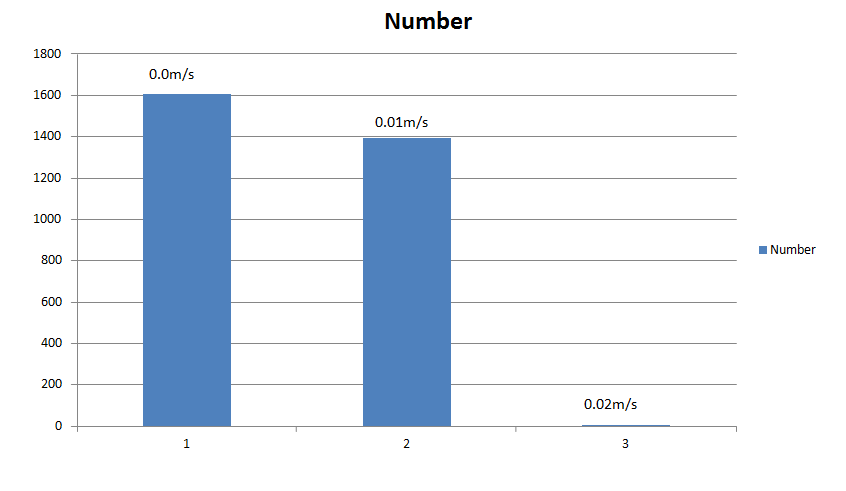
\includegraphics[width=1\textwidth]
{graph/evaluation.png}
\caption{Processing time of our approach.}
\label{fig:evaluation}
\end{figure}
The median time compared to the median time of folowgraphs appoach introduced in chapter \ref{chap:3}. The evaluation of  folowgraphs appoach was performed on a 2.4 GHz Quad Core Desktop PC with 4G of memory, running 32-bit Windows Vista Home Premium with Service Pack 1\cite{silvio}. The result was shown in figure \ref{fig:evaluation1}. The median time to perform classification was 0.25 seconds. The slowest sample that is required 5.12 seconds. Only 6 samples required more than 2 seconds. Processing time of followgraph approach was shown in figure \ref{fig:evaluation2}.
\begin{figure}[h!]
\centering
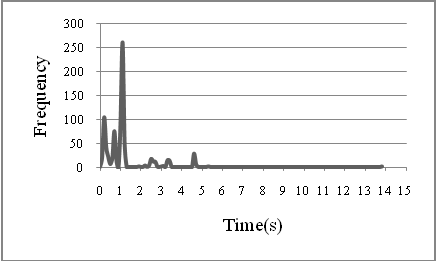
\includegraphics[width=1\textwidth]
{graph/evaluation1.png}
\caption{Processing time of followgraphs approach.}
\label{fig:evaluation1}
\end{figure}

According to the median time to perform classification, the system implemented by our approach is faster than the malware classification based on the followgraphs approach.
\section{Discussion}
\subsubsection{Accuracy evaluation}
Obviously, in experiment we obtained 4181 malware samples for constructing decision tree and 255 malware samples for evaluating system. The accuracy of our malware classification system is 57\%. However, the accuracy of Mota, Waledac, Sality samples are too low because the number of those samples is less than Virut, or IRC bot samples. There are 2243 Virut, and 1169 IRC bot samples. Otherwise, there is only 79 Mota, 61 Waledac, 66 Sality samples.

The number of Downadup samples in training data are small, but the accuracy of Downadup samples are higher than another. The reasons is Downadup binary files are different to other families so that decision tree easily identify Downadup samples.  

Moreover, all of Gaobot samples is classified into IRC bot because the Gaobot binary file is nearly similar to IRC bot.

\subsubsection{Efficiency of classification}

1606 malware samples required approximately 0 seconds. With our approach, malware samples use meta-data to compare with each node of decision tree. In some case, malware sample is only correspond to one to two node in decision tree so that the result is exported instantly. 
The result of processing shows that our approach is faster than followgraphs approach. 




\chapter{Conclusion}\label{chap:7}
\section{Conclusion}
A vast amount of new malware sample each day is the difficult problem in malware analysis. Our malware fast malware classification system is successful to classify unknown malware into malware family which have semantic characteristic. We strongly believe that our system is useful for malware analysis to determine malware behavior and semantic malware characteristic to more easily analyze a vast amount of malware.
However, there is a problem that our system use only malware meta-data and cannot detect the malware family which have same program structure.\\
Surprisingly, our system cannot be used to classify W32 malware which does not have the signature of PE file signature. 
 
\section{Future work}
Our system successfully classified unknown malware into malware family. In the future work, we use Windows API in order to make our system determined unknown malware into the malware families, which have similarity of program structure. 



% ------------------------------------
% --- frontmatter: Acknowledgement ---
% ------------------------------------
\newpage
\pagenumbering{roman}   % define page number in roman style
\setcounter{page}{1}    % start page numbering
\section*{Acknowledgement}

First and foremost, I am sincerely grateful to faculty members in Murai and Tokuda Laboratory, Professor Hideyuki Tokuda, Professor Jun Murai, Associate Professor Hiroyuki Kusumoto, Professor Osamu Nakamura, Associate Professor Kazunori Takashio, Assistant Professor Noriyuki Shigechika, Assistant Professor Rodney D. Van Meter III, Associate Professor Keisuke Uehara, Associate Professor Jin Mitsugi, Lecturer Jin Nakazawa.

I would be extremely thankful to Professor Keiji Takeda for his endless help and valuable comments to my thesis. Without his help, I cannot even think of writing this thesis.

I own my special thank to Doctor Masayoshi Mizutani for his sincerely help and many advices since the time I first came to the lab.

I would like to thank to Master Kunihiko Shigematsu, Yuki Uehara, my friend Toshinori Usui, for listening	and giving me many useful discussion points. Their gentleness and encouragement helped me overcome many hard times in this one year. 
 
I would also like to thank all ISC group members, Sega-kun, Alc-kun, Lushe-kun, Nobita-kun, Fuyuki-kun, Yoshi-kun, Asp-chan, Hino-kun, Rocky-kun, Vigo-kun, who have given me numerous support and always cheer me up in my hard times. 

I would like to thank to members in Murai and Tokuda Laboratory who have been so friendly and kindly supporting me with my research.




% ----------------
% --- appendix ---
% ----------------
\appendix

% literature

\newpage
\addcontentsline{toc}{chapter}{References}
\bibliography{reference/literature}



% --------------------------------------------
% --- last page: Declaration of Authorship ---
% --------------------------------------------

%\newpage
%\thispagestyle{empty}
%%{\Large{\bf Declaration of Authorship}}\vspace{0.5cm}

\section*{Declaration of Authorship}

I hereby confirm that I have authored this Bachelor's/Master's
thesis independently and without use of others than the indicated
sources. All passages which are literally or in general matter
taken out of publications or other sources are marked as such.
\vspace{1cm}

Berlin, September 30, 2007 \vspace{0.5cm}

your name (and signature, of course)





\end{document}
